%!TEX root = ../thesis.tex

\section{実験の手順}

\begin{figure}[h]
  \centering
  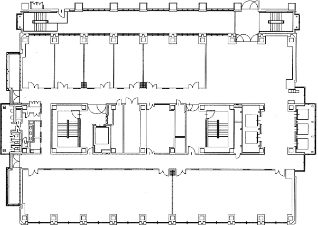
\includegraphics[keepaspectratio, scale=0.80] {images/RobotGuidance_cit3f.png}
  \captionsetup{justification=raggedright} % キャプションを左寄せに
  \caption{The environment of the experiment}
  \label{Fig:RobotGuidance_cit3f}
\end{figure}

\begin{figure}[h]
  \centering
  \begin{minipage}[c]{65mm} 
      \centering
      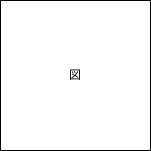
\includegraphics[height=40mm]{images/figure.png}
      \subcaption{hoge}
  \end{minipage}
  \begin{minipage}[c]{65mm} 
      \centering
      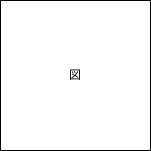
\includegraphics[height=40mm]{images/figure.png}
      \subcaption{hoge}
  \end{minipage}
  \caption{hogehoge}
  \label{Fig:4.1hoge}
\end{figure}

\newpage
